\documentclass{article}

%---------------------------------------
% Packages and Color Definitions
%---------------------------------------
\usepackage{amsmath}
\usepackage{amsfonts}
\usepackage{tikz}
\usepackage{xcolor}
\usepackage{pagecolor}

% Dark background with light text
\definecolor{darkbg}{HTML}{1E1E1E}
\definecolor{lighttext}{HTML}{D4D4D4}
\pagecolor{darkbg}
\color{lighttext}

%---------------------------------------
% Document Title (heading) info
%---------------------------------------
\title{Neural-Network Backpropagation Notes}
\author{anomitroid}
\date{\today}

%---------------------------------------
% Document Begins
%---------------------------------------
\begin{document}

\maketitle

%=======================================
\section{Gradient Descent}
%=======================================

\subsection{Finite Difference Definition}\label{sec:finite-difference}

\noindent The derivative of a cost function \(C(w)\) with respect to parameter \(w\) is defined via the limit of the finite-difference quotient. Explicitly, we write:
\begin{align}
    C'(w)
    &= \lim_{\epsilon \to 0} \frac{C(w + \epsilon) - C(w)}{\epsilon}
\end{align}
\noindent Here:
\begin{itemize}
    \item \(C(w + \epsilon)\) is the cost evaluated at \(w + \epsilon\).
    \item \(C(w)\) is the cost at \(w\).
    \item Dividing by \(\epsilon\) gives the average rate of change over the interval \([w,\,w+\epsilon]\).
    \item Taking \(\epsilon \to 0\) yields the instantaneous rate of change, i.e.\ the derivative.
\end{itemize}

\vspace{1em}

\subsection{Linear Regression Cost and Its Derivative}\label{sec:linear-regression}

\noindent Consider a simple linear model with weight \(w\), input \(x_i\), and true output \(y_i\).  The mean-squared error (MSE) cost over \(n\) examples is:
\begin{align}
    C(w) 
    &= \frac{1}{n} \sum_{i=1}^{n} {\bigl(x_i \,w \;-\; y_i\bigr)}^2
\end{align}
We want to compute \(\frac{dC}{dw}\).  To do so, we proceed step by step.

%---------------------------------------
\subsubsection{Step 1: Distribute the Derivative over the Sum}\label{sec:linreg-step1}

\noindent First note that
\[
    C(w) 
    = \frac{1}{n} \sum_{i=1}^{n} f_i(w), 
    \quad\text{where}\quad 
    f_i(w) = {\bigl(x_i w - y_i\bigr)}^2
\]
By linearity of differentiation,
\begin{align}
    \frac{dC}{dw}
    &= \frac{d}{dw} \biggl(\frac{1}{n} \sum_{i=1}^{n} f_i(w)\biggr) 
    = \frac{1}{n} \sum_{i=1}^{n} \frac{d}{dw}\bigl[f_i(w)\bigr]
    \label{eq:linear-sum-rule}
\end{align}
\noindent Here, we have used:
\begin{itemize}
    \item \(\tfrac{d}{dw}\bigl(\sum_{i=1}^n f_i(w)\bigr) = \sum_{i=1}^n \tfrac{d}{dw}[f_i(w)]\)
    \item The constant factor \(1/n\) can be pulled outside the derivative.
\end{itemize}

\vspace{0.5em}

%---------------------------------------
\subsubsection{Step 2: Differentiate Each Term}\label{sec:linreg-step2}

\noindent We now focus on a single term:
\[
    f_i(w) = {\bigl(x_i w - y_i\bigr)}^2
\]
By the chain rule, if \(g(w) = {\bigl(x_i w - y_i\bigr)}^2\), then
\[
    \frac{d}{dw} g(w)
    = 2\,(x_i w - y_i)\;\cdot\;\frac{d}{dw}\bigl(x_i w - y_i\bigr)
\]
\noindent Next, since \(\frac{d}{dw}(x_i w - y_i) = x_i\), we have
\begin{align}
    \frac{d}{dw}{\bigl(x_i w - y_i\bigr)}^2
    &= 2\,(x_i w - y_i)\;\bigl(x_i\bigr)
    \label{eq:linreg-chain}
\end{align}
\noindent Substituting back into\eqref{eq:linear-sum-rule}, we get:
\begin{align}
    \frac{dC}{dw}
    &= \frac{1}{n} \sum_{i=1}^{n} \Bigl[\,2\,(x_i w - y_i)\,x_i\Bigr]
\end{align}

\vspace{0.5em}

\noindent Finally, we can factor out the \(2\) if desired:
\begin{align}
    \frac{dC}{dw}
    &= \frac{2}{n} \sum_{i=1}^{n} (x_i w - y_i)\,x_i
    \label{eq:linreg-final}
\end{align}
\noindent This expression gives the gradient of the MSE cost with respect to \(w\).  

%=======================================
\section{One-Neuron Model}
%=======================================

\noindent In this section, we analyze a single neuron (sigmoid activation) with first one input, then two inputs.  We present:
\begin{enumerate}
    \item Forward-pass equations
    \item Detailed derivation of \(\sigma(z)\) and \(\sigma'(z)\)
    \item Cost function and step-by-step computation of gradients
\end{enumerate}

%---------------------------------------
\subsection{Single Input Neuron}\label{sec:one-neuron-single-input}
%---------------------------------------

\subsubsection{Network Diagram and Forward Pass}\label{sec:one-neuron-forward}

\noindent A single input \(x\) is multiplied by weight \(w\), added to bias \(b\), and passed through a sigmoid activation to produce output \(a\).  The diagram is:

\begin{center}
    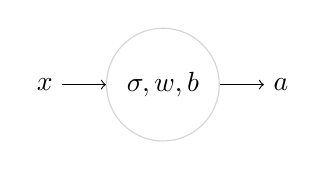
\begin{tikzpicture}[baseline=(N.center)]
        \def\d{1.5}
        % Nodes
        \node (X) at (-\d, 0) {\(x\)};
        \node[shape=circle, draw=lighttext, inner sep=0.5em] (N) at (0,0) {\(\sigma, w, b\)};
        \node (Y) at (\d,0) {\(a\)};
        % Arrows
        \path[->] (X) edge (N);
        \path[->] (N) edge (Y);
    \end{tikzpicture}
\end{center}

\noindent Therefore, the forward-pass equation is:
\begin{align}
    z 
    &= x\,w + b, 
    \quad
    a \;=\; \sigma(z)
    \label{eq:one-neuron-forward}
\end{align}
\noindent We will omit the intermediate \(z\) in later notation and write \(a = \sigma(x w + b)\).

%---------------------------------------
\subsubsection{Sigmoid Activation and Its Derivative}\label{sec:one-neuron-sigmoid}
%---------------------------------------

\noindent The sigmoid activation function is defined by:
\begin{align}
    \sigma(z) 
    &= \frac{1}{1 + e^{-z}}
    \label{eq:sigmoid-def}
\end{align}

\vspace{0.5em}
\noindent To find \(\sigma'(z)\), we apply the chain rule.  Let
\[
    h(z) = \frac{1}{1 + e^{-z}} = {(1 + e^{-z})}^{-1}
\]
Then
\[
    \frac{dh}{dz} 
    = -1 \cdot {(1 + e^{-z})}^{-2} \;\cdot\; \frac{d}{dz}[\,1 + e^{-z}\,]
\]
Since \(\frac{d}{dz}[\,1 + e^{-z}\,] = -\,e^{-z}\), we obtain:
\begin{align}
    \sigma'(z) 
    &= - {(1 + e^{-z})}^{-2} \;\cdot\; \bigl(-\,e^{-z}\bigr)
    = \frac{e^{-z}}{{(1 + e^{-z})}^2}
    \label{eq:sigmoid-deriv1}
\end{align}

\noindent Next, we rewrite \(\frac{e^{-z}}{{(1 + e^{-z})}^2}\) in terms of \(\sigma(z)\). Observe:
\[
    \sigma(z) = \frac{1}{1 + e^{-z}}
    \quad\Longrightarrow\quad
    1 - \sigma(z) = 1 - \frac{1}{1 + e^{-z}}
    = \frac{(1 + e^{-z}) - 1}{1 + e^{-z}}
    = \frac{e^{-z}}{1 + e^{-z}}
\]
Hence,
\[
    \sigma(z) \,\bigl(1 - \sigma(z)\bigr)
    = \frac{1}{1 + e^{-z}} \;\cdot\; \frac{e^{-z}}{1 + e^{-z}}
    = \frac{e^{-z}}{{(1 + e^{-z})}^2}
\]
Comparing with\eqref{eq:sigmoid-deriv1}, we conclude:
\begin{align}
    \sigma'(z) 
    &= \sigma(z)\,\bigl[1 - \sigma(z)\bigr]
    \label{eq:sigmoid-deriv2}
\end{align}

%---------------------------------------
\subsubsection{Cost Function and Gradients}\label{sec:one-neuron-gradient}
%---------------------------------------

\noindent Given a dataset \({\{(x_i,\,y_i)\}}_{i=1}^n\), the neuron's output for the \(i\)th example is:
\[
    a_i = \sigma(x_i w + b)
\]
We define the MSE cost as:
\begin{align}
    C(w, b)
    &= \frac{1}{n} \sum_{i=1}^{n} {\bigl(a_i - y_i\bigr)}^2
    \label{eq:one-neuron-cost}
\end{align}
To apply gradient descent, we need \(\partial C / \partial w\) and \(\partial C / \partial b\).  We compute these in detail.

%---------------------------------------
\paragraph{Gradient with respect to \(w\)\\}\label{sec:grad-w-one-neuron}

\noindent First, note that
\[
    C(w, b) 
    = \frac{1}{n}\sum_{i=1}^{n} {\bigl(a_i - y_i\bigr)}^2,
    \quad
    a_i = \sigma(x_i w + b)
\]
We differentiate \(C\) with respect to \(w\) using the chain rule:

\begin{align}
    \frac{\partial C}{\partial w}
    &= \frac{\partial}{\partial w} \biggl(\frac{1}{n}\sum_{i=1}^{n} {(a_i - y_i)}^2\biggr)
    = \frac{1}{n} \sum_{i=1}^{n} \frac{\partial}{\partial w} {\bigl(a_i - y_i\bigr)}^2
    \label{eq:one-grad-step1}
\end{align}

\noindent Focus on a single summand:
\[
    \frac{\partial}{\partial w} {\bigl(a_i - y_i\bigr)}^2
    = 2\,\bigl(a_i - y_i\bigr)\;\cdot\; \frac{\partial}{\partial w}\bigl(a_i - y_i\bigr)
\]
Since \(y_i\) is a constant (true label), \(\frac{\partial}{\partial w}(a_i - y_i) = \frac{\partial a_i}{\partial w}\).  Therefore,
\begin{align}
    \frac{\partial}{\partial w} {\bigl(a_i - y_i\bigr)}^2
    &= 2\,\bigl(a_i - y_i\bigr)\;\cdot\;\frac{\partial a_i}{\partial w}
    \label{eq:one-grad-step2}
\end{align}

\noindent Next, compute \(\frac{\partial a_i}{\partial w}\).  Recall \(a_i = \sigma(z_i)\) with \(z_i = x_i w + b\).  By the chain rule:
\begin{align}
    \frac{\partial a_i}{\partial w}
    &= \sigma'(z_i)\;\cdot\;\frac{\partial}{\partial w}(z_i)
    = \sigma'(x_i w + b)\;\cdot\; x_i
    \label{eq:one-grad-step3a}
\end{align}
Using\eqref{eq:sigmoid-deriv2}, \(\sigma'(x_i w + b) = a_i\,\bigl(1 - a_i\bigr)\).  Hence,
\begin{align}
    \frac{\partial a_i}{\partial w}
    &= a_i\,\bigl(1 - a_i\bigr)\,x_i
    \label{eq:one-grad-step3b}
\end{align}

\noindent Substitute\eqref{eq:one-grad-step3b} into\eqref{eq:one-grad-step2}:
\begin{align}
    \frac{\partial}{\partial w} {\bigl(a_i - y_i\bigr)}^2
    &= 2\,(a_i - y_i)\;\bigl[a_i\,\bigl(1 - a_i\bigr)\,x_i\bigr]
\end{align}
Finally, plug back into\eqref{eq:one-grad-step1}:
\begin{align}
    \frac{\partial C}{\partial w}
    &= \frac{1}{n} \sum_{i=1}^{n} \Bigl[\,2\,(a_i - y_i)\,a_i\,(1 - a_i)\,x_i\Bigr]
    = \frac{2}{n} \sum_{i=1}^{n} (a_i - y_i)\,a_i\,(1 - a_i)\,x_i
    \label{eq:one-grad-w-final}
\end{align}

%---------------------------------------
\paragraph{Gradient with respect to \(b\)\\}\label{sec:grad-b-one-neuron}

\noindent Similarly, to find \(\partial C / \partial b\), start with\eqref{eq:one-neuron-cost}:
\[
    \frac{\partial C}{\partial b}
    = \frac{\partial}{\partial b} \biggl(\frac{1}{n}\sum_{i=1}^{n}{(a_i - y_i)}^2\biggr)
    = \frac{1}{n} \sum_{i=1}^{n} \frac{\partial}{\partial b}{(a_i - y_i)}^2
\]
By the same reasoning as before,
\begin{align}
    \frac{\partial}{\partial b} {(a_i - y_i)}^2
    &= 2\,(a_i - y_i)\;\cdot\;\frac{\partial}{\partial b}(a_i - y_i),
    \label{eq:one-grad-b-step1}
\end{align}
and since \(\frac{\partial}{\partial b}(a_i - y_i) = \frac{\partial a_i}{\partial b}\), we compute:
\begin{align}
    \frac{\partial a_i}{\partial b}
    &= \sigma'(x_i w + b)\;\cdot\;\frac{\partial}{\partial b}(x_i w + b)
    = a_i\,(1 - a_i)\;\cdot\; 1
    = a_i\,(1 - a_i)
    \label{eq:one-grad-b-step2}
\end{align}
Thus,
\[
    \frac{\partial}{\partial b} {(a_i - y_i)}^2
    = 2\,(a_i - y_i)\;\bigl[a_i\,(1 - a_i)\bigr],
\]
and finally,
\begin{align}
    \frac{\partial C}{\partial b}
    &= \frac{1}{n} \sum_{i=1}^{n} \Bigl[\,2\,(a_i - y_i)\,a_i\,(1 - a_i)\Bigr]
    = \frac{2}{n} \sum_{i=1}^{n} (a_i - y_i)\,a_i\,(1 - a_i)
    \label{eq:one-grad-b-final}
\end{align}

%=======================================
\section{One-Neuron Model with Two Inputs}
%=======================================

\noindent Now we extend the single-input neuron to accept two inputs \(x\) and \(u\), with weights \(w_1\) and \(w_2\), and bias \(b\).  

%---------------------------------------
\subsection{Network Diagram and Forward Pass}\label{sec:one-neuron-two-inputs}
%---------------------------------------

\noindent The architecture is:

\begin{center}
    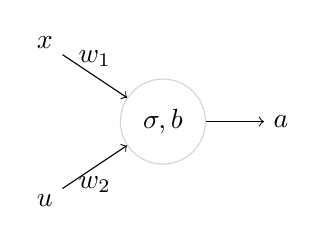
\begin{tikzpicture}[baseline=(N.center)]
        \def\d{1.5}
        % Nodes
        \node (X) at (-\d,  \d/ \d) {\(x\)};
        \node (U) at (-\d, -\d/ \d) {\(u\)};
        \node[shape=circle, draw=lighttext, inner sep=0.5em] (N) at (0,0) {\(\sigma, b\)};
        \node (Z) at (\d,0) {\(a\)};
        % Arrows with weight labels
        \path[->] (X) edge node[above]{\(w_1\)} (N);
        \path[->] (U) edge node[below]{\(w_2\)} (N);
        \path[->] (N) edge (Z);
    \end{tikzpicture}
\end{center}

\noindent The forward-pass is:
\begin{align}
    z 
    &= x\,w_1 \;+\; u\,w_2 \;+\; b, 
    \quad
    a = \sigma(z)
    \label{eq:two-input-forward}
\end{align}
\noindent Again, we abbreviate \(a = \sigma(x w_1 + u w_2 + b)\)

\vspace{0.5em}
\noindent Recall from\eqref{eq:sigmoid-def} and\eqref{eq:sigmoid-deriv2}:
\[
    \sigma(z) = \frac{1}{1 + e^{-z}}, 
    \quad
    \sigma'(z) = \sigma(z)\,(1 - \sigma(z))
\]

%---------------------------------------
\subsubsection{Cost Function and Gradient Details}\label{sec:two-input-gradient}
%---------------------------------------

\noindent Given data \({\{(x_i,\,u_i,\,z_i)\}}_{i=1}^n\), the predicted output is:
\[
    a_i = \sigma(x_i w_1 + u_i w_2 + b)
\]
The cost is:
\begin{align}
    C(w_1,\,w_2,\,b)
    &= \frac{1}{n} \sum_{i=1}^{n} {\bigl(a_i - z_i\bigr)}^2
    \label{eq:two-input-cost}
\end{align}
We compute each partial derivative step by step.

%---------------------------------------
\paragraph{Gradient with respect to \(w_1\)\\}\label{sec:grad-w1-two-input}

\noindent Start with:
\begin{align}
    \frac{\partial C}{\partial w_1}
    &= \frac{\partial}{\partial w_1} \biggl(\frac{1}{n}\sum_{i=1}^{n}{{(a_i - z_i)}}^2\biggr)
    = \frac{1}{n} \sum_{i=1}^{n} \frac{\partial}{\partial w_1}{{(a_i - z_i)}}^2
    \label{eq:two-grad-w1-step1}
\end{align}
For each \(i\), apply the chain rule:
\begin{align}
    \frac{\partial}{\partial w_1} {{(a_i - z_i)}}^2
    &= 2\,{(a_i - z_i)}\;\cdot\;\frac{\partial}{\partial w_1}{(a_i - z_i)}
    = 2\,{(a_i - z_i)}\;\cdot\;\frac{\partial a_i}{\partial w_1}
    \label{eq:two-grad-w1-step2}
\end{align}
Next, \(\frac{\partial a_i}{\partial w_1}\) is found by chain rule on \(a_i = \sigma(z_i)\) with \(z_i = x_i w_1 + u_i w_2 + b\):
\begin{align}
    \frac{\partial a_i}{\partial w_1}
    &= \sigma'(z_i)\;\cdot\;\frac{\partial}{\partial w_1}(z_i)
    = \sigma'(x_i w_1 + u_i w_2 + b)\;\cdot\; x_i \\
    &= a_i\,\bigl(1 - a_i\bigr)\,x_i
    \label{eq:two-grad-w1-step3}
\end{align}
Combining\eqref{eq:two-grad-w1-step2} and\eqref{eq:two-grad-w1-step3}:
\[
    \frac{\partial}{\partial w_1}{(a_i - z_i)}^2
    = 2\,{(a_i - z_i)}\;\bigl[a_i\,(1 - a_i)\,x_i\bigr]
\]
Therefore, from\eqref{eq:two-grad-w1-step1}:
\begin{align}
    \frac{\partial C}{\partial w_1}
    &= \frac{1}{n} \sum_{i=1}^{n} \Bigl[\,2\,{(a_i - z_i)}\,a_i\,(1 - a_i)\,x_i\Bigr]
    = \frac{2}{n} \sum_{i=1}^{n} {(a_i - z_i)}\,a_i\,(1 - a_i)\,x_i
    \label{eq:two-grad-w1-final}
\end{align}

%---------------------------------------
\paragraph{Gradient with respect to \(w_2\)\\}\label{sec:grad-w2-two-input}

\noindent Analogously,
\begin{align}
    \frac{\partial C}{\partial w_2}
    &= \frac{\partial}{\partial w_2} \biggl(\frac{1}{n}\sum_{i=1}^{n}{(a_i - z_i)}^2\biggr)
    = \frac{1}{n} \sum_{i=1}^{n} \frac{\partial}{\partial w_2}{(a_i - z_i)}^2
    \label{eq:two-grad-w2-step1}
\end{align}
For each term:
\begin{align}
    \frac{\partial}{\partial w_2} {(a_i - z_i)}^2
    &= 2\,{(a_i - z_i)}\;\cdot\;\frac{\partial a_i}{\partial w_2},
    \label{eq:two-grad-w2-step2}
\end{align}
and
\begin{align}
    \frac{\partial a_i}{\partial w_2}
    &= \sigma'(x_i w_1 + u_i w_2 + b)\;\cdot\;\frac{\partial}{\partial w_2}(x_i w_1 + u_i w_2 + b)
    = a_i\,(1 - a_i)\;\cdot\; u_i
    \label{eq:two-grad-w2-step3}
\end{align}
Thus,
\[
    \frac{\partial}{\partial w_2}{(a_i - z_i)}^2
    = 2\,{(a_i - z_i)}\,\bigl[a_i\,(1 - a_i)\,u_i\bigr]
\]
Hence from\eqref{eq:two-grad-w2-step1}:
\begin{align}
    \frac{\partial C}{\partial w_2}
    &= \frac{1}{n} \sum_{i=1}^{n} \Bigl[\,2\,{(a_i - z_i)}\,a_i\,(1 - a_i)\,u_i\Bigr]
    = \frac{2}{n} \sum_{i=1}^{n} {(a_i - z_i)}\,a_i\,(1 - a_i)\,u_i
    \label{eq:two-grad-w2-final}
\end{align}

%---------------------------------------
\paragraph{Gradient with respect to \(b\)\\}\label{sec:grad-b-two-input}

\noindent Finally, for \(b\):
\begin{align}
    \frac{\partial C}{\partial b}
    &= \frac{\partial}{\partial b} \biggl(\frac{1}{n}\sum_{i=1}^{n}{(a_i - z_i)}^2\biggr)
    = \frac{1}{n} \sum_{i=1}^{n} \frac{\partial}{\partial b}{(a_i - z_i)}^2
    \label{eq:two-grad-b-step1}
\end{align}
Each term:
\begin{align}
    \frac{\partial}{\partial b} {(a_i - z_i)}^2
    &= 2\,{(a_i - z_i)}\;\cdot\;\frac{\partial a_i}{\partial b},
    \label{eq:two-grad-b-step2}
\end{align}
and
\begin{align}
    \frac{\partial a_i}{\partial b}
    &= \sigma'(x_i w_1 + u_i w_2 + b)\;\cdot\;\frac{\partial}{\partial b}(x_i w_1 + u_i w_2 + b)
    = a_i\,(1 - a_i)\;\cdot\;1
    = a_i\,(1 - a_i)
    \label{eq:two-grad-b-step3}
\end{align}
Hence,
\[
    \frac{\partial}{\partial b} {(a_i - z_i)}^2
    = 2\,{(a_i - z_i)}\,\bigl[a_i\,(1 - a_i)\bigr],
\]
and from\eqref{eq:two-grad-b-step1}:
\begin{align}
    \frac{\partial C}{\partial b}
    &= \frac{1}{n} \sum_{i=1}^{n} \Bigl[\,2\,{(a_i - z_i)}\,a_i\,(1 - a_i)\Bigr]
    = \frac{2}{n} \sum_{i=1}^{n} {(a_i - z_i)}\,a_i\,(1 - a_i)
    \label{eq:two-grad-b-final}
\end{align}

\vspace{1em}
\noindent With these detailed intermediate steps, the derivations for both the single-input neuron and the two-input neuron are now fully transparent.

%---------------------------------------
% Two-Neuron Model with One Input (Detailed Backprop)
%---------------------------------------
\section{Two-Neuron Model with One Input}\label{sec:two-neuron}

In this section, we consider a network with one input \(x\) that feeds into two sequential neurons (a hidden layer of size 1 and an output neuron).  We provide a fully detailed derivation of the forward pass, cost function, and backpropagation steps, showing every derivative calculation and explaining the role of each term (including the concept of “error”).

%---------------------------------------
\subsection{Network Architecture and Forward Pass}\label{sec:two-neuron-forward}

\noindent The architecture can be drawn as:

\begin{center}
    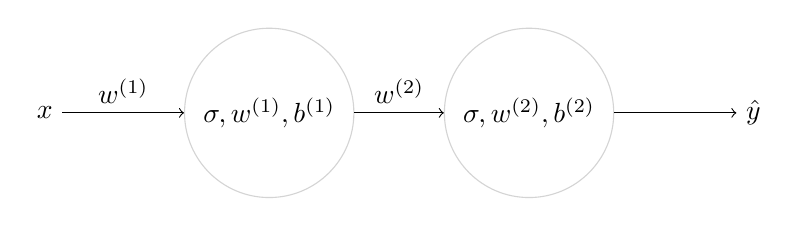
\begin{tikzpicture}[baseline=(N2.center)]
        \def\d{1.5}
        % Input node
        \node (X) at (-3*\d, 0) {$x$};
        % Hidden neuron 1
        \node[shape=circle, draw=lighttext, inner sep=0.5em] (N1) at (-1.1 * \d, 0) {$\sigma, w^{(1)}, b^{(1)}$};
        % Output neuron 2
        \node[shape=circle, draw=lighttext, inner sep=0.5em] (N2) at (1.1 * \d, 0) {$\sigma, w^{(2)}, b^{(2)}$};
        % Output node
        \node (Y) at (3*\d, 0) {$\hat y$};
        % Arrows
        \path[->] (X) edge node[above] {$w^{(1)}$} (N1);
        \path[->] (N1) edge node[above] {$w^{(2)}$} (N2);
        \path[->] (N2) edge (Y);
    \end{tikzpicture}
\end{center}

\noindent We index examples by \(i = 1,2,\dots,n\).  For the \(i\)-th example:

\begin{itemize}
    \item The input is \(x_i\).
    \item The hidden layer pre-activation (``net input'') is 
    \[
        z_i^{(1)} = x_i\,w^{(1)} + b^{(1)}
    \]
    \item The hidden layer activation (output of neuron 1) is 
    \[
        a_i^{(1)} = \sigma\bigl(z_i^{(1)}\bigr) \,=\, \sigma\bigl(x_i\,w^{(1)} + b^{(1)}\bigr)
    \]
    \item The output layer pre-activation is 
    \[
        z_i^{(2)} = a_i^{(1)}\,w^{(2)} + b^{(2)}
    \]
    \item The final prediction (activation of neuron 2) is 
    \[
        a_i^{(2)} = \hat y_i = \sigma\bigl(z_i^{(2)}\bigr) \,=\, \sigma\bigl(a_i^{(1)}\,w^{(2)} + b^{(2)}\bigr)
    \]
\end{itemize}

\noindent In summary:
\begin{align}
    z_i^{(1)} &= x_i\,w^{(1)} + b^{(1)}, \\
    a_i^{(1)} &= \sigma\bigl(z_i^{(1)}\bigr), \\
    z_i^{(2)} &= a_i^{(1)}\,w^{(2)} + b^{(2)}, \\
    a_i^{(2)} &= \sigma\bigl(z_i^{(2)}\bigr).
\end{align}

\noindent Here, \(\sigma(z) = 1/(1 + e^{-z})\) is the sigmoid activation (see Sections~\ref{sec:one-neuron-sigmoid} for its definition and derivative).  Note the superscripts \((1)\) and \((2)\) indicate layer index.

%---------------------------------------
\subsection{Cost Function}\label{sec:two-neuron-cost}

\noindent Given target labels \(y_i\) for each example, we define the mean-squared error (MSE) over the training set:
\begin{align}
    C\bigl(w^{(1)}, b^{(1)}, w^{(2)}, b^{(2)}\bigr)
    &= \frac{1}{n} \sum_{i=1}^{n} {\bigl(a_i^{(2)} - y_i\bigr)}^2
    \label{eq:two-cost}
\end{align}

\noindent Our goal is to compute the four gradients:
\(\partial C/\partial w^{(1)},\; \partial C/\partial b^{(1)},\; \partial C/\partial w^{(2)},\; \partial C/\partial b^{(2)}\).
These tell us how to update each parameter to decrease the cost.

%---------------------------------------
\subsection{Backpropagation: Definitions and ``Error'' Terms}\label{sec:two-neuron-backprop-definitions}

\noindent The key idea of backpropagation is to compute derivatives of the cost \(C\) with respect to each parameter by recursively applying the chain rule from the output layer back toward the input.

\paragraph{Output-Layer ``Error'' (\(\delta_i^{(2)}\))\\}
We define the error at the output neuron for example \(i\) as:
\[
    \delta_i^{(2)} \;=\; \frac{\partial C}{\partial z_i^{(2)}}
\]
Intuitively, \(\delta_i^{(2)}\) measures how much the cost changes if we perturb the pre-activation \(z_i^{(2)}\) at the output neuron.  A large \(|\delta_i^{(2)}|\) means that a small change in \(z_i^{(2)}\) will cause a large change in cost.

Using the chain rule, we can write:
\[
    \delta_i^{(2)} = \frac{\partial C}{\partial a_i^{(2)}} \cdot \frac{\partial a_i^{(2)}}{\partial z_i^{(2)}}
\]
We compute each factor separately:

\begin{enumerate}
    \item \(\displaystyle {\frac{\partial C}{\partial a_i^{(2)}}:}\)  From\eqref{eq:two-cost},
    \[
        C = \frac{1}{n} \sum_{j=1}^n {\bigl(a_j^{(2)} - y_j\bigr)}^2
    \]
    Differentiating with respect to \(a_i^{(2)}\) (only the \(j=i\) term survives):
    \[
        \frac{\partial C}{\partial a_i^{(2)}}
        = \frac{1}{n} \cdot 2\,{\bigl(a_i^{(2)} - y_i\bigr)}
        = \frac{2}{n}\,{\bigl(a_i^{(2)} - y_i\bigr)}
    \]
    This term represents the discrepancy between the network's output \(a_i^{(2)}\) and the true label \(y_i\).  We sometimes call 
    \(\bigl(a_i^{(2)} - y_i\bigr)\) the 
    \emph{prediction error} at the output.

    \item \(\displaystyle {\frac{\partial a_i^{(2)}}{\partial z_i^{(2)}}:}\)  Since \(a_i^{(2)} = \sigma(z_i^{(2)})\) and \(\sigma'(z) = \sigma(z)(1 - \sigma(z))\) (see\eqref{eq:sigmoid-deriv2}),
    \[
        \frac{\partial a_i^{(2)}}{\partial z_i^{(2)}}
        = \sigma'\bigl(z_i^{(2)}\bigr)
        = a_i^{(2)}\bigl(1 - a_i^{(2)}\bigr)
    \]
    This factor tells us how sensitive the activation is to changes in the pre-activation.
\end{enumerate}

\noindent Combining these:
\begin{align}
    \delta_i^{(2)}
    &= \frac{\partial C}{\partial a_i^{(2)}} \;\cdot\; \frac{\partial a_i^{(2)}}{\partial z_i^{(2)}} \\
    &= \Bigl[\tfrac{2}{n}\,(a_i^{(2)} - y_i)\Bigr]\ \cdot\ \bigl[a_i^{(2)}(1 - a_i^{(2)})\bigr] \\
    &= \frac{2}{n}\,(a_i^{(2)} - y_i)\;a_i^{(2)}(1 - a_i^{(2)})
    \label{eq:delta2}
\end{align}

\noindent In many implementations, one omits the factor \(2/n\) by absorbing it into the learning rate; however, for full transparency, we keep it here.

\paragraph{Hidden-Layer ``Error'' (\(\delta_i^{(1)}\))\\}
We similarly define the error for the hidden neuron:
\[
    \delta_i^{(1)} \;=\; \frac{\partial C}{\partial z_i^{(1)}}
\]
To relate \(\delta_i^{(1)}\) back to \(\delta_i^{(2)}\), we apply the chain rule through the output neuron:

\[
    \delta_i^{(1)}
    = \frac{\partial C}{\partial z_i^{(1)}}
    = \frac{\partial C}{\partial a_i^{(2)}} \cdot \frac{\partial a_i^{(2)}}{\partial z_i^{(2)}} \cdot \frac{\partial z_i^{(2)}}{\partial a_i^{(1)}} \cdot \frac{\partial a_i^{(1)}}{\partial z_i^{(1)}}
\]
Notice that \(C\) depends on \(z_i^{(1)}\) only through \(a_i^{(1)}\) and \(z_i^{(2)}\).  We can group these into known terms:

\begin{itemize}
    \item We already computed \(\displaystyle \frac{\partial C}{\partial a_i^{(2)}} = \frac{2}{n}(a_i^{(2)} - y_i)\)
    \item We already computed \(\displaystyle \frac{\partial a_i^{(2)}}{\partial z_i^{(2)}} = a_i^{(2)}(1 - a_i^{(2)})\)
    \item \(\displaystyle \frac{\partial z_i^{(2)}}{\partial a_i^{(1)}} = w^{(2)}\), since \(z_i^{(2)} = a_i^{(1)} w^{(2)} + b^{(2)}\)
    \item \(\displaystyle \frac{\partial a_i^{(1)}}{\partial z_i^{(1)}} = \sigma'(z_i^{(1)}) = a_i^{(1)}(1 - a_i^{(1)})\)
\end{itemize}

\noindent Therefore,
\begin{align}
    \delta_i^{(1)}
    &= \Bigl[\frac{2}{n}\,(a_i^{(2)} - y_i)\Bigr] \cdot \bigl[a_i^{(2)}(1 - a_i^{(2)})\bigr] \cdot w^{(2)} \cdot \bigl[a_i^{(1)}(1 - a_i^{(1)})\bigr] \\
    &= \Bigl[\frac{2}{n}(a_i^{(2)} - y_i)\,a_i^{(2)}(1 - a_i^{(2)})\,w^{(2)}\Bigr]\ \cdot\ \bigl[a_i^{(1)}(1 - a_i^{(1)})\bigr]
    \label{eq:delta1}
\end{align}

\noindent Here, \(\delta_i^{(1)}\) quantifies the contribution of the hidden neuron's pre-activation \(z_i^{(1)}\) to the overall cost.  It is the “backpropagated” error from the output neuron, scaled by the derivative of the hidden activation.

%---------------------------------------
\subsection{Gradients for All Parameters}\label{sec:two-neuron-gradients}

\noindent Once we have \(\delta_i^{(2)}\) and \(\delta_i^{(1)}\), we can obtain parameter gradients by noting how each parameter appears in the pre-activations.

\subsubsection{Gradient w.r.t. Output-Layer Parameters}\label{sec:grad-output}

\paragraph{Gradient of \(C\) w.r.t.\ \(w^{(2)}\)\\}
Since \(z_i^{(2)} = a_i^{(1)} w^{(2)} + b^{(2)}\), we have
\[
    \frac{\partial z_i^{(2)}}{\partial w^{(2)}} = a_i^{(1)}
\]
By definition of \(\delta_i^{(2)} = \partial C/\partial z_i^{(2)}\), the chain rule gives:
\[
    \frac{\partial C}{\partial w^{(2)}}
    = \sum_{i=1}^{n} \frac{\partial C}{\partial z_i^{(2)}} \cdot \frac{\partial z_i^{(2)}}{\partial w^{(2)}}
    = \sum_{i=1}^{n} \delta_i^{(2)} \;\bigl[a_i^{(1)}\bigr]
\]
Since we included a factor of \(1/n\) in \(\delta_i^{(2)}\) (see\eqref{eq:delta2}), we write:
\begin{align}
    \frac{\partial C}{\partial w^{(2)}}
    &= \sum_{i=1}^{n} \delta_i^{(2)} \,a_i^{(1)}
    \label{eq:grad-w2}
\end{align}

\paragraph{Gradient of \(C\) w.r.t.\ \(b^{(2)}\)\\}
Since \(z_i^{(2)} = a_i^{(1)} w^{(2)} + b^{(2)}\),
\[
    \frac{\partial z_i^{(2)}}{\partial b^{(2)}} = 1
\]
Hence,
\begin{align}
    \frac{\partial C}{\partial b^{(2)}}
    &= \sum_{i=1}^{n} \delta_i^{(2)} \cdot 1
    = \sum_{i=1}^{n} \delta_i^{(2)}
    \label{eq:grad-b2}
\end{align}

\subsubsection{Gradient w.r.t. Hidden-Layer Parameters}\label{sec:grad-hidden}

\paragraph{Gradient of \(C\) w.r.t.\ \(w^{(1)}\)\\}
Since \(z_i^{(1)} = x_i w^{(1)} + b^{(1)}\), we have
\[
    \frac{\partial z_i^{(1)}}{\partial w^{(1)}} = x_i
\]
By the chain rule,
\[
    \frac{\partial C}{\partial w^{(1)}}
    = \sum_{i=1}^{n} \frac{\partial C}{\partial z_i^{(1)}} \cdot \frac{\partial z_i^{(1)}}{\partial w^{(1)}}
    = \sum_{i=1}^{n} \delta_i^{(1)} \;\bigl[x_i\bigr]
\]
Thus,
\begin{align}
    \frac{\partial C}{\partial w^{(1)}}
    &= \sum_{i=1}^{n} \delta_i^{(1)}\,x_i
    \label{eq:grad-w1}
\end{align}

\paragraph{Gradient of \(C\) w.r.t.\ \(b^{(1)}\)\\}
Since \(z_i^{(1)} = x_i w^{(1)} + b^{(1)}\),
\[
    \frac{\partial z_i^{(1)}}{\partial b^{(1)}} = 1
\]
Therefore,
\begin{align}
    \frac{\partial C}{\partial b^{(1)}}
    &= \sum_{i=1}^{n} \delta_i^{(1)}
    \label{eq:grad-b1}
\end{align}

%---------------------------------------
\subsection{Step-by-Step Derivative Computations}\label{sec:two-neuron-stepwise}

\paragraph{1. Compute \(\partial C/\partial a_i^{(2)}\)\\}
From \(C = \tfrac{1}{n}\sum_{j}{(a_j^{(2)} - y_j)}^2\),
\[
    \frac{\partial C}{\partial a_i^{(2)}}
    = \frac{1}{n} \cdot 2\,(a_i^{(2)} - y_i)
    = \frac{2}{n}\,(a_i^{(2)} - y_i)
\]

\paragraph{2. Compute \(\partial a_i^{(2)}/\partial z_i^{(2)}\)\\}
Since \(a_i^{(2)} = \sigma(z_i^{(2)})\) with \(\sigma'(z) = \sigma(z)(1 - \sigma(z))\),
\[
    \frac{\partial a_i^{(2)}}{\partial z_i^{(2)}} = a_i^{(2)}\bigl(1 - a_i^{(2)}\bigr)
\]

\paragraph{3. Form \(\delta_i^{(2)} = \partial C/\partial z_i^{(2)}\)\\}
By chain rule,
\[
    \delta_i^{(2)} = \frac{\partial C}{\partial a_i^{(2)}} \cdot \frac{\partial a_i^{(2)}}{\partial z_i^{(2)}}
    = \Bigl[\frac{2}{n}(a_i^{(2)} - y_i)\Bigr]\ \cdot\ \bigl[a_i^{(2)}(1 - a_i^{(2)})\bigr]
\]

\paragraph{4. Compute \(\partial C/\partial w^{(2)}\) and \(\partial C/\partial b^{(2)}\)\\}
Since \(z_i^{(2)} = a_i^{(1)}w^{(2)} + b^{(2)}\):
\[
    \frac{\partial z_i^{(2)}}{\partial w^{(2)}} = a_i^{(1)},
    \quad
    \frac{\partial z_i^{(2)}}{\partial b^{(2)}} = 1
\]
Hence,
\[
    \frac{\partial C}{\partial w^{(2)}} = \sum_i \delta_i^{(2)}\,a_i^{(1)},
    \quad
    \frac{\partial C}{\partial b^{(2)}} = \sum_i \delta_i^{(2)}
\]

\paragraph{5. Compute \(\partial z_i^{(2)}/\partial a_i^{(1)}\)\\}
Since \(z_i^{(2)} = a_i^{(1)} w^{(2)} + b^{(2)}\),
\[
    \frac{\partial z_i^{(2)}}{\partial a_i^{(1)}} = w^{(2)}
\]

\paragraph{6. Compute \(\partial a_i^{(1)}/\partial z_i^{(1)}\)\\}
Since \(a_i^{(1)} = \sigma(z_i^{(1)})\),
\[
    \frac{\partial a_i^{(1)}}{\partial z_i^{(1)}} = a_i^{(1)}\bigl(1 - a_i^{(1)}\bigr)
\]

\paragraph{7. Form \(\delta_i^{(1)} = \partial C/\partial z_i^{(1)}\)\\}
By combining steps 1--6 using chain rule:
\begin{align*}
    \delta_i^{(1)}
    &= \frac{\partial C}{\partial a_i^{(2)}} \cdot \frac{\partial a_i^{(2)}}{\partial z_i^{(2)}} \cdot \frac{\partial z_i^{(2)}}{\partial a_i^{(1)}} \cdot \frac{\partial a_i^{(1)}}{\partial z_i^{(1)}} \\
    &= \Bigl[\frac{2}{n}(a_i^{(2)} - y_i)\Bigr]\ \cdot\ \bigl[a_i^{(2)}(1 - a_i^{(2)})\bigr]\ \cdot\ w^{(2)} \ \cdot\ \bigl[a_i^{(1)}(1 - a_i^{(1)})\bigr].
\end{align*}

\paragraph{8. Compute \(\partial C/\partial w^{(1)}\) and \(\partial C/\partial b^{(1)}\)\\}
Since \(z_i^{(1)} = x_i w^{(1)} + b^{(1)}\):
\[
    \frac{\partial z_i^{(1)}}{\partial w^{(1)}} = x_i,
    \quad
    \frac{\partial z_i^{(1)}}{\partial b^{(1)}} = 1
\]
Therefore:
\[
    \frac{\partial C}{\partial w^{(1)}} = \sum_i \delta_i^{(1)}\,x_i,
    \quad
    \frac{\partial C}{\partial b^{(1)}} = \sum_i \delta_i^{(1)}
\]

%---------------------------------------
\subsection{Interpretation of ``Error'' Terms}\label{sec:two-neuron-error-interpretation}

\begin{itemize}
    \item \textbf{Output error \(\delta_i^{(2)}\):}  Measures how much changing the output neuron's pre-activation \(z_i^{(2)}\) affects the cost.  It combines:
    \begin{enumerate}
        \item The 
        prediction error \((a_i^{(2)} - y_i)\), which tells us how far the network's output is from the target.
        \item The factor \(a_i^{(2)}(1 - a_i^{(2)})\), which is the derivative of the sigmoid and scales the error by the local slope of the activation.
        \item The factor \(2/n\), which normalizes by dataset size and accounts for the derivative of \({(\cdot)}^2\).
    \end{enumerate}

    \item \textbf{Hidden error \(\delta_i^{(1)}\):}  Measures how much changing the hidden neuron's pre-activation \(z_i^{(1)}\) affects the final cost.  It arises by “backpropagating” the output error through:
    \begin{enumerate}
        \item The weight \(w^{(2)}\), since the hidden neuron's activation \(a_i^{(1)}\) contributes to \(z_i^{(2)}\) via \(w^{(2)}\).
        \item The sigmoid slope at the hidden layer \(a_i^{(1)}(1 - a_i^{(1)})\), since that is \(\partial a_i^{(1)}/\partial z_i^{(1)}\).
    \end{enumerate}
    In effect, \(\delta_i^{(1)}\) redistributes the output-layer error back into the hidden layer, scaled by how sensitive the hidden activation is.
\end{itemize}

\noindent By computing these errors \(\delta^{(2)}\) and \(\delta^{(1)}\), we efficiently obtain all parameter gradients using\eqref{eq:grad-w2}–\eqref{eq:grad-b1}.  This is the essence of backpropagation: local gradients at each neuron (the ``error'' terms) are combined with the derivatives of pre-activations to give global parameter gradients.

%---------------------------------------
% End of Two-Neuron Detailed Section
%---------------------------------------

%=======================================
\section{One-Input, \(\boldsymbol{n}\)-Layer Neural Network}\label{sec:one-input-n-layers}
%=======================================



\noindent In this section, we generalize from the specific ``two-layer' (one hidden layer + one output layer) case to an arbitrary number \(n\) of layers, all with a single scalar input \(x\). We will:
\begin{enumerate}
    \item Introduce notation for \(n\) layers.
    \item Describe the forward pass in full detail.
    \item Define the cost function (mean-squared error) over a dataset.
    \item Derive the backpropagation formulas layer by layer, showing every intermediate term.
    \item Explain the meaning of each symbol and each mathematical step.
\end{enumerate}

\vspace{0.5em}
\noindent Throughout, we keep the dark-background / light-text style established earlier.

%---------------------------------------
\subsection{Architecture and Notation}\label{sec:nlayers-architecture}
%---------------------------------------

\noindent Consider a neural network with one input \(x\in\mathbb{R}\) (a single scalar), followed by \(n-1\) hidden layers and one final output layer. We index layers by superscript \((\ell)\), where \(\ell = 1,2,\dots,n\). Layer \(\ell=1\) is the very first layer that directly receives the input \(x\), and layer \(\ell = n\) is the output layer whose activation we compare to the true label.

\vspace{0.5em}
\noindent For each layer \(\ell\), we have:
\begin{itemize}
    \item A \emph{weight} \(w^{(\ell)}\in\mathbb{R}\) (since each layer receives exactly one scalar input from the previous layer, there is exactly one weight per layer).
    \item A \emph{bias} \(b^{(\ell)}\in\mathbb{R}\).
    \item A \emph{pre-activation} \(z^{(\ell)}\in\mathbb{R}\), defined just before applying the activation function.
    \item An \emph{activation} \(a^{(\ell)} = \sigma\bigl(z^{(\ell)}\bigr)\) (we will use the sigmoid nonlinearity by default, though any differentiable activation could be used).
\end{itemize}

\noindent In summary:
\[
    \begin{aligned}
        &\underbrace{x}_{\text{input}} 
        \xrightarrow{\;w^{(1)},\,b^{(1)}\;}
        \underbrace{z^{(1)}}_{\text{pre-act. 1}}
        \xrightarrow{\sigma}
        \underbrace{a^{(1)}}_{\text{act. 1}}
        \xrightarrow{\;w^{(2)},\,b^{(2)}\;}
        z^{(2)} \xrightarrow{\sigma} a^{(2)}
        \;\cdots\;
        \xrightarrow{\;w^{(n)},\,b^{(n)}\;}
        z^{(n)} \xrightarrow{\sigma} a^{(n)} = \hat{y}
    \end{aligned}
\]

\noindent Here:
\begin{itemize}
    \item \(z^{(1)} = x\,w^{(1)} + b^{(1)}\).  
    \item For \(\ell = 2,3,\dots,n\), 
    \[
      z^{(\ell)} = a^{(\ell-1)}\,w^{(\ell)} + b^{(\ell)}.
    \]
    \item The final network output (prediction) is \(a^{(n)} = \hat{y}\).  
    \item The true label for example \(i\) is \(y_i\).  
\end{itemize}

\vspace{1em}
\noindent \textbf{Illustration of a One-Input, \(n\)-Layer Network}

\begin{center}
    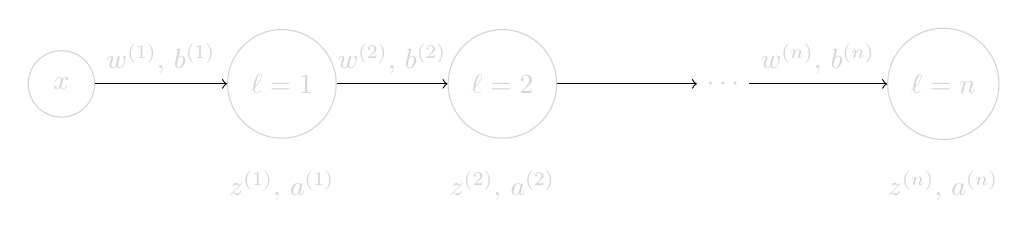
\begin{tikzpicture}[node distance=1.8cm, every node/.style={text=lighttext}]
        % Input node
        \node (x) [draw=lighttext, circle, inner sep=0.6em] {\(x\)};
        % Layer 1 node
        \node (L1) [draw=lighttext, circle, right of=x, xshift=1cm, inner sep=0.6em] 
            {\(\ell=1\)};
        % Layer 2 node
        \node (L2) [draw=lighttext, circle, right of=L1, xshift=1cm, inner sep=0.6em] 
            {\(\ell=2\)};
        % Dots
        \node (dots) [right of=L2, xshift=1cm] {\(\cdots\)};
        % Layer n node
        \node (Ln) [draw=lighttext, circle, right of=dots, xshift=1cm, inner sep=0.6em] 
            {\(\ell=n\)};
        
        % Arrows between layers
        \path[->] (x) edge node[above] {\(w^{(1)},\,b^{(1)}\)} (L1);
        \path[->] (L1) edge node[above] {\(w^{(2)},\,b^{(2)}\)} (L2);
        \path[->] (L2) edge (dots);
        \path[->] (dots) edge node[above] {\(w^{(n)},\,b^{(n)}\)} (Ln);
        
        % Labels for pre-activation and activation
        \node [below of=L1, yshift=0.5cm] {\(z^{(1)},\,a^{(1)}\)};
        \node [below of=L2, yshift=0.5cm] {\(z^{(2)},\,a^{(2)}\)};
        \node [below of=Ln, yshift=0.5cm] {\(z^{(n)},\,a^{(n)}\)};
    \end{tikzpicture}
\end{center}

\noindent In this diagram:
\begin{itemize}
    \item The single input \(x\) feeds into layer \(\ell=1\), producing pre-activation \(z^{(1)}\) and activation \(a^{(1)}\).  
    \item That activation \(a^{(1)}\) becomes the input to layer \(\ell=2\), producing \(z^{(2)},\,a^{(2)}\).  
    \item This process continues through \(\ell=3,4,\dots,n\).  
    \item The final output \(a^{(n)}\) is the network's prediction \(\hat{y}\).  
\end{itemize}

\vspace{0.5em}
\noindent We now detail the forward pass, cost, and backward pass (backpropagation).

\vspace{0.5em}
\noindent We assume a dataset of \(N\) examples \({\{(x_i,\,y_i)\}}_{i=1}^N\).  We will drop the index \(i\) during the derivation, writing \((x,y)\) for a generic single example, and re-insert the sum at the end to define the full cost.

%---------------------------------------
\subsection{Forward Pass}\label{sec:nlayers-forward}
%---------------------------------------

\noindent For a single example \((x,y)\), the forward-pass proceeds layer by layer:

\begin{enumerate}
    \item \textbf{Layer \(\ell = 1\):}  
    \[
      z^{(1)} = w^{(1)}\,x \;+\; b^{(1)}, 
      \qquad
      a^{(1)} = \sigma\bigl(z^{(1)}\bigr).
    \]
    \noindent Here \(\sigma\) is the sigmoid function:
    \[
      \sigma(u) \;=\; \frac{1}{1 + e^{-\,u}}.
    \]
    \item \textbf{Layer \(\ell = 2\):} 
    \[
      z^{(2)} = w^{(2)}\,a^{(1)} \;+\; b^{(2)}, 
      \qquad
      a^{(2)} = \sigma\bigl(z^{(2)}\bigr).
    \]
    \item \(\quad\vdots\)
    \item \textbf{Layer \(\ell = n\) (Output Layer):} 
    \[
      z^{(n)} = w^{(n)}\,a^{(n-1)} \;+\; b^{(n)}, 
      \qquad
      a^{(n)} = \sigma\bigl(z^{(n)}\bigr) \;=\; \hat{y}.
    \]
\end{enumerate}

\noindent Each \(z^{(\ell)}\) is called the \emph{pre-activation}, and each \(a^{(\ell)}\) is called the \emph{activation} of layer \(\ell\).  Note that \(a^{(0)} := x\) if we wish to unify notation, but we will keep \(x\) as a special symbol.

\vspace{0.5em}
\noindent In full, for our one-input \(n\)-layer network,
\[
\begin{aligned}
    z^{(1)} &= w^{(1)}\,x + b^{(1)}, & a^{(1)} &= \sigma\bigl(z^{(1)}\bigr),\\
    z^{(2)} &= w^{(2)}\,a^{(1)} + b^{(2)}, & a^{(2)} &= \sigma\bigl(z^{(2)}\bigr),\\
    &\;\;\;\vdots &&\;\;\;\vdots\\
    z^{(n)} &= w^{(n)}\,a^{(n-1)} + b^{(n)}, & a^{(n)} &= \sigma\bigl(z^{(n)}\bigr) = \hat{y}.
\end{aligned}
\]

\vspace{0.5em}
\noindent After computing \(a^{(n)}\), we measure the discrepancy against the true label \(y\) via a loss function.  We choose the mean-squared error (MSE) for a single example:
\[
    L\bigl(x,y; \{w^{(\ell)},b^{(\ell)}\}\bigr)
    = {\bigl(a^{(n)} - y\bigr)}^2.
\]

%---------------------------------------
\subsection{Cost over the Entire Dataset}\label{sec:nlayers-cost}
%---------------------------------------

\noindent To train, we average the loss over all \(N\) examples:
\begin{align}
    C 
    &= \frac{1}{N}\sum_{i=1}^{N} L\bigl(x_i,\,y_i;\,\{w^{(\ell)},b^{(\ell)}\}\bigr) \nonumber\\
    &= \frac{1}{N}\sum_{i=1}^{N} {\bigl(\hat{y}_i - y_i\bigr)}^2 
    = \frac{1}{N}\sum_{i=1}^{N} {\Bigl[a_i^{(n)} - y_i\Bigr]}^2.
    \label{eq:nlayers-full-cost}
\end{align}

\noindent Here \(\hat{y}_i = a_i^{(n)}\) is the network's prediction on input \(x_i\).  The goal of training is to find weights and biases \({\{w^{(\ell)},b^{(\ell)}\}}_{\ell=1}^n\) that minimize \(C\).

---

%---------------------------------------
\subsection{Backpropagation: Detailed Derivation}\label{sec:nlayers-backprop}
%---------------------------------------

\noindent We now derive how to compute 
\(\displaystyle \frac{\partial C}{\partial w^{(\ell)}}, \; \frac{\partial C}{\partial b^{(\ell)}}\) 
for \(\ell = 1,2,\ldots,n\).  Because the network is built by repeated compositions, we apply the chain rule systematically from the output layer backward to the input layer.  For clarity, we focus on a single example \((x,y)\) and then re-insert the sum over \(i\) at the end—this is equivalent to computing \(\partial L/\partial\theta\) for one example, then averaging.

\vspace{0.5em}
\noindent \textbf{Step 1: Define ``Error' at the Output Layer.}

Recall the single-example loss
\[
    L 
    = {\bigl(a^{(n)} - y\bigr)}^2,
    \qquad
    a^{(n)} = \sigma\bigl(z^{(n)}\bigr).
\]
We introduce the shorthand
\[
    \delta^{(n)} \;=\; \frac{\partial L}{\partial z^{(n)}}.
\]
That is, \(\delta^{(n)}\) measures how much the loss \(L\) changes if we nudge the pre-activation \(z^{(n)}\) at the output layer.  By the chain rule:
\[
    \delta^{(n)} 
    = \frac{\partial L}{\partial a^{(n)}} 
      \;\cdot\; \frac{\partial a^{(n)}}{\partial z^{(n)}}.
\]
We compute each factor:
\begin{itemize}
    \item \(\displaystyle \frac{\partial L}{\partial a^{(n)}} 
      = \frac{\partial}{\partial a^{(n)}} {(a^{(n)} - y)}^2 
      = 2\,\bigl(a^{(n)} - y\bigr)\)
    \item \(\displaystyle \frac{\partial a^{(n)}}{\partial z^{(n)}} 
      = \sigma'\bigl(z^{(n)}\bigr) 
      = \sigma\bigl(z^{(n)}\bigr)\,\bigl[1 - \sigma\bigl(z^{(n)}\bigr)\bigr] 
      = a^{(n)}\,\bigl(1 - a^{(n)}\bigr)\)
\end{itemize}
Therefore,
\begin{align}
    \delta^{(n)} 
    &= \Bigl[2\,\bigl(a^{(n)} - y\bigr)\Bigr] 
       \times \Bigl[a^{(n)}\,(1 - a^{(n)})\Bigr] 
    = 2\,\bigl(a^{(n)} - y\bigr)\,a^{(n)}\,(1 - a^{(n)}).
    \label{eq:delta-output}
\end{align}

\vspace{0.5em}
\noindent \textbf{Step 2: Gradients at the Output Layer.}

For layer \(\ell = n\), the pre-activation was
\[
    z^{(n)} = w^{(n)}\,a^{(n-1)} + b^{(n)}.
\]
Hence:
\begin{itemize}
    \item \(\displaystyle \frac{\partial z^{(n)}}{\partial w^{(n)}} 
       = a^{(n-1)}\),
    \item \(\displaystyle \frac{\partial z^{(n)}}{\partial b^{(n)}} 
       = 1\)
\end{itemize}
By the chain rule for the loss:
\begin{align}
    \frac{\partial L}{\partial w^{(n)}} 
    &= \frac{\partial L}{\partial z^{(n)}} 
       \;\cdot\; \frac{\partial z^{(n)}}{\partial w^{(n)}} 
    = \delta^{(n)} \;\times\; a^{(n-1)},
    \label{eq:grad-wn} 
    \\
    \frac{\partial L}{\partial b^{(n)}} 
    &= \frac{\partial L}{\partial z^{(n)}} 
       \;\cdot\; \frac{\partial z^{(n)}}{\partial b^{(n)}} 
    = \delta^{(n)} \;\times\; 1 
    = \delta^{(n)}.
    \label{eq:grad-bn} 
\end{align}

\vspace{0.5em}
\noindent \textbf{Step 3: Propagate Error Back to Hidden Layers.}

For a generic hidden layer \(\ell\) (where \(1 \le \ell \le n-1\)), we define
\[
    \delta^{(\ell)} \;=\; \frac{\partial L}{\partial z^{(\ell)}}.
\]
We will derive a recurrence expressing \(\delta^{(\ell)}\) in terms of \(\delta^{(\ell+1)}\).  First, observe that
\[
    a^{(\ell)} = \sigma\bigl(z^{(\ell)}\bigr),
    \qquad
    z^{(\ell+1)} = w^{(\ell+1)}\,a^{(\ell)} + b^{(\ell+1)}.
\]
Hence, by the multivariate chain rule:
\[
    \delta^{(\ell)} 
    = \frac{\partial L}{\partial z^{(\ell)}} 
    = \frac{\partial L}{\partial z^{(\ell+1)}} 
      \;\cdot\; \frac{\partial z^{(\ell+1)}}{\partial a^{(\ell)}} 
      \;\cdot\; \frac{\partial a^{(\ell)}}{\partial z^{(\ell)}}.
\]
We already know:
\[
    \frac{\partial L}{\partial z^{(\ell+1)}} = \delta^{(\ell+1)}, 
    \qquad
    \frac{\partial z^{(\ell+1)}}{\partial a^{(\ell)}} 
    = w^{(\ell+1)},
    \qquad
    \frac{\partial a^{(\ell)}}{\partial z^{(\ell)}} 
    = \sigma'\bigl(z^{(\ell)}\bigr) 
    = a^{(\ell)}\,(1 - a^{(\ell)}).
\]
Therefore, for \(\ell = n-1,\,n-2,\,\dots,\,1\):
\begin{align}
    \delta^{(\ell)} 
    &= \delta^{(\ell+1)} \; \times\; w^{(\ell+1)} \; \times\; \bigl[a^{(\ell)}\,\bigl(1 - a^{(\ell)}\bigr)\bigr] 
    = \bigl[w^{(\ell+1)}\,\delta^{(\ell+1)}\bigr]\;a^{(\ell)}\bigl(1 - a^{(\ell)}\bigr).
    \label{eq:delta-hidden}
\end{align}

\noindent In words:
\[
    \delta^{(\ell)} = \bigl(\text{next-layer error } \delta^{(\ell+1)}\bigr) 
                     \times \bigl(\text{weight } w^{(\ell+1)}\bigr) 
                     \times \bigl(\text{activation slope } a^{(\ell)}(1 - a^{(\ell)})\bigr).
\]
Geometrically, \(\delta^{(\ell)}\) measures how much the final loss \(L\) would change if you nudge the pre-activation at layer \(\ell\).  We compute these \(\delta^{(\ell)}\) in a backward sweep from \(\ell = n\) down to \(\ell = 1\).

\vspace{0.5em}
\noindent \textbf{Step 4: Gradients for Hidden Layers.}

Once \(\delta^{(\ell)}\) is known, the gradient of \(L\) with respect to \(w^{(\ell)}\) and \(b^{(\ell)}\) is straightforward, because
\[
    z^{(\ell)} = w^{(\ell)}\,a^{(\ell-1)} + b^{(\ell)} \quad (\text{with }a^{(0)} := x).
\]
Thus:
\begin{align}
    \frac{\partial L}{\partial w^{(\ell)}} 
    &= \frac{\partial L}{\partial z^{(\ell)}} 
       \;\cdot\; \frac{\partial z^{(\ell)}}{\partial w^{(\ell)}} 
    = \delta^{(\ell)} \;\times\; a^{(\ell-1)}, 
    \label{eq:grad-wl} 
    \\
    \frac{\partial L}{\partial b^{(\ell)}} 
    &= \frac{\partial L}{\partial z^{(\ell)}} 
       \;\cdot\; \frac{\partial z^{(\ell)}}{\partial b^{(\ell)}} 
    = \delta^{(\ell)} \;\times\; 1 
    = \delta^{(\ell)}.
    \label{eq:grad-bl} 
\end{align}
Here \(a^{(\ell-1)}\) is the activation coming \emph{into} layer \(\ell\).  For \(\ell = 1\), \(a^{(0)} = x\) (the network's input).

\vspace{0.5em}
\noindent \textbf{Step 5: Summing / Averaging Over All Examples.}

All of the above was for a single example \((x,y)\).  To get the gradient of the total cost \(C\) in\eqref{eq:nlayers-full-cost}, we average the single-example gradients:
\[
    \frac{\partial C}{\partial w^{(\ell)}} 
    = \frac{1}{N} \sum_{i=1}^N 
      \frac{\partial L_i}{\partial w^{(\ell)}}, 
    \qquad
    \frac{\partial C}{\partial b^{(\ell)}} 
    = \frac{1}{N} \sum_{i=1}^N 
      \frac{\partial L_i}{\partial b^{(\ell)}},
\]
where \(L_i = {\bigl(a_i^{(n)} - y_i\bigr)}^2\) is the loss on example \(i\).  In practice, one often uses mini-batch gradients, but the principle is identical: compute \(\delta_i^{(\ell)}\) for each example \(i\), then average across that batch.

\vspace{0.5em}
\noindent Putting it all together:

\begin{enumerate}
    \item \textbf{Forward Pass (per example \(i\)):}  
      \[
      \begin{aligned}
        z_i^{(1)} &= w^{(1)}\,x_i \;+\; b^{(1)}, 
        &a_i^{(1)} &= \sigma\bigl(z_i^{(1)}\bigr),\\
        z_i^{(2)} &= w^{(2)}\,a_i^{(1)} \;+\; b^{(2)}, 
        &a_i^{(2)} &= \sigma\bigl(z_i^{(2)}\bigr),\\
        &\;\;\;\vdots &&\;\;\;\vdots\\
        z_i^{(n)} &= w^{(n)}\,a_i^{(n-1)} \;+\; b^{(n)}, 
        &a_i^{(n)} &= \sigma\bigl(z_i^{(n)}\bigr).
      \end{aligned}
      \]
      Then \(L_i = {\bigl(a_i^{(n)} - y_i\bigr)}^2\)

    \item \textbf{Compute Output-Layer Error \(\delta_i^{(n)}\):}  
      \[
        \delta_i^{(n)} 
        = 2\,\bigl(a_i^{(n)} - y_i\bigr)\;a_i^{(n)}\bigl(1 - a_i^{(n)}\bigr).
      \]

    \item \textbf{Backward Pass (for \(\ell = n-1,n-2,\dots,1\)):}  
      \[
        \delta_i^{(\ell)} 
        = \bigl[w^{(\ell+1)}\,\delta_i^{(\ell+1)}\bigr] 
          \times a_i^{(\ell)}\bigl(1 - a_i^{(\ell)}\bigr).
      \]

    \item \textbf{Gradients (per example \(i\)):}  
      For each \(\ell = 1,2,\dots,n\),
      \begin{align*}
        \frac{\partial L_i}{\partial w^{(\ell)}} 
        &= \delta_i^{(\ell)} \;\times\; a_i^{(\ell-1)}, 
        \quad 
          \text{(where)}a_i^{(0)} = x_i\text{}; \\
        \frac{\partial L_i}{\partial b^{(\ell)}} 
        &= \delta_i^{(\ell)}.
      \end{align*}

    \item \textbf{Average Over All \(N\) Examples:}  
      \[
        \frac{\partial C}{\partial w^{(\ell)}} 
        = \frac{1}{N}\sum_{i=1}^N \frac{\partial L_i}{\partial w^{(\ell)}}, 
        \qquad
        \frac{\partial C}{\partial b^{(\ell)}} 
        = \frac{1}{N}\sum_{i=1}^N \frac{\partial L_i}{\partial b^{(\ell)}}.
      \]
\end{enumerate}

---

%---------------------------------------
\subsection{Key Explanations and Interpretations}\label{sec:nlayers-explanations}
%---------------------------------------

\noindent We summarize the conceptual meaning of each term:

\begin{itemize}
    \item \textbf{Pre-activation \(z^{(\ell)}\):}  
      This is the weighted input plus bias for layer \(\ell\).  It is the argument to the activation function at that layer.

    \item \textbf{Activation \(a^{(\ell)}\):}  
      Defined by \(a^{(\ell)} = \sigma\bigl(z^{(\ell)}\bigr)\).  This is what layer \(\ell\) passes forward to layer \(\ell+1\).  For \(\ell=0\), we set \(a^{(0)} = x\).

    \item \textbf{Single-example loss \(L = {(a^{(n)} - y)}^2\):}  
      Measures how far the network's prediction \(a^{(n)}\) is from the true label \(y\).

    \item \textbf{Error term \(\delta^{(n)}\) at the output:}  
      \[
        \delta^{(n)} = \frac{\partial L}{\partial z^{(n)}} 
                     = 2\,(a^{(n)} - y)\,\sigma'\bigl(z^{(n)}\bigr).
      \]
      This quantity tells us how sensitive the loss is to a small change in \(z^{(n)}\).  Since \(z^{(n)}\) is the input of the output neuron, \(\delta^{(n)}\) measures the “blame” placed on that neuron's pre-activation.

    \item \textbf{Error term \(\delta^{(\ell)}\) at a hidden layer \(\ell < n\):}  
      \[
        \delta^{(\ell)} 
        = w^{(\ell+1)}\,\delta^{(\ell+1)} \;\times\; \sigma'\bigl(z^{(\ell)}\bigr).
      \]
      Here, \(w^{(\ell+1)}\,\delta^{(\ell+1)}\) carries back how much layer \(\ell+1\) “blamed” layer \(\ell\).  Multiplying by \(\sigma'(z^{(\ell)})\) captures how a small perturbation in \(z^{(\ell)}\) changes \(a^{(\ell)}\), and thus the final loss.

    \item \textbf{Gradients \(\partial L/\partial w^{(\ell)}\) and \(\partial L/\partial b^{(\ell)}\):}  
      Once \(\delta^{(\ell)}\) is known, we simply note that 
      \[
        z^{(\ell)} = w^{(\ell)}\,a^{(\ell-1)} + b^{(\ell)} 
        \quad\Longrightarrow\quad
        \frac{\partial z^{(\ell)}}{\partial w^{(\ell)}} = a^{(\ell-1)}, 
        \quad
        \frac{\partial z^{(\ell)}}{\partial b^{(\ell)}} = 1.
      \]
      Hence 
      \[
        \frac{\partial L}{\partial w^{(\ell)}} 
        = \delta^{(\ell)}\,a^{(\ell-1)}, 
        \qquad
        \frac{\partial L}{\partial b^{(\ell)}} 
        = \delta^{(\ell)}.
      \]
      In other words, \(\delta^{(\ell)}\) is the ``rate of change of loss with respect to a small change in {\(z^{(\ell)}\),}'' and \(a^{(\ell-1)}\) is the input to \(z^{(\ell)}\).  

    \item \textbf{Averaging over examples:}  
      When using the mean-squared error over \(N\) examples, each example yields its own \(\delta_i^{(\ell)}\).  We average the per-example gradients to find \(\partial C/\partial w^{(\ell)}\).  
\end{itemize}

\vspace{0.5em}
\noindent Because every step uses only quantities computed in the forward pass (activations \(a^{(\ell)}\)) and previously computed \(\delta\) values (one from the layer above), backpropagation requires exactly one forward sweep and one backward sweep per mini-batch.  No repeated forward passes are needed per parameter, which is what makes deep network training computationally feasible even when \(n\) is large.

---

%---------------------------------------
% End of new section on 1-input, n-layer network
%---------------------------------------

%=======================================
\section{Arbitrary \(\boldsymbol{n}\) Inputs and \(\boldsymbol{L}\) Layers}\label{sec:n-inputs-layers}
%=======================================

\noindent In this section, we extend our analysis to a fully general feedforward neural network with:
\begin{itemize}
    \item \(n\) \emph{input features} \(x \in \mathbb{R}^n\).
    \item \(L\) \emph{layers} (numbered \(\ell = 1,2,\dots,L\)), each of which may contain an arbitrary number of neurons.
\end{itemize}
We will:
\begin{enumerate}
    \item Introduce notation for arbitrary input dimension and a sequence of hidden/output layers.
    \item Describe the forward pass in a vectorized, scalable form.
    \item Define the dataset cost (mean-squared error) and explain how it depends on the network's parameters.
    \item Derive the backpropagation formulas in full detail, layer by layer, showing every intermediate step.
    \item Clarify the dimensions and interpretations of all vectors and matrices.
\end{enumerate}

\medskip
\noindent Throughout, we continue using a dark background with light text; new notation is bolded for clarity.

%---------------------------------------
\subsection{Network Architecture and Notation}\label{sec:n-inputs-layers-architecture}
%---------------------------------------

\noindent Let \(x \in \mathbb{R}^n\) be the column vector of \(n\) input features:
\[
    x = \begin{pmatrix}x_{1}\\x_{2}\\\vdots\\x_{n}\end{pmatrix}.
\]
We build an \(L\)-layer feedforward network as follows:

\begin{itemize}
    \item \(\ell=0\) denotes the \emph{input layer}, whose “activation” is simply \(a^{(0)} = x \in \mathbb{R}^n\).
    \item For each layer \(\ell = 1,2,\dots,L\), we denote:
    \begin{itemize}
        \item \(m_{\ell}\) = number of neurons in layer \(\ell\).  
              We allow \(m_{1},m_{2},\dots,m_{L}\) to be arbitrary positive integers.  
        \item \(\mathbf{W}^{(\ell)} \in \mathbb{R}^{\,m_{\ell}\times m_{\ell-1}}\) = weight matrix connecting layer \(\ell-1\) to layer \(\ell\).  
        \item \(\mathbf{b}^{(\ell)} \in \mathbb{R}^{\,m_{\ell}}\) = bias vector for layer \(\ell\).  
        \item \(\mathbf{z}^{(\ell)} \in \mathbb{R}^{\,m_{\ell}}\) = pre-activation vector for layer \(\ell\).  
        \item \(\mathbf{a}^{(\ell)} \in \mathbb{R}^{\,m_{\ell}}\) = activation vector for layer \(\ell\), with \(\mathbf{a}^{(\ell)} = \sigma\bigl(\mathbf{z}^{(\ell)}\bigr)\) applied elementwise.
    \end{itemize}
    \item The final layer \(\ell = L\) is the \emph{output layer}. If the task is regression with a single scalar output, then \(m_{L} = 1\). If it is multiclass classification, \(m_{L}\) can be larger; here we assume \(m_{L}\) may be arbitrary.
\end{itemize}

\noindent Concretely, for each layer \(\ell = 1,2,\dots,L\):
\[
    \mathbf{z}^{(\ell)}
    \;=\; \mathbf{W}^{(\ell)}\,\mathbf{a}^{(\ell-1)} \;+\; \mathbf{b}^{(\ell)},
    \qquad
    \mathbf{a}^{(\ell)}
    \;=\; \sigma\bigl(\mathbf{z}^{(\ell)}\bigr),
\]
where \(\sigma(\cdot)\) acts component-wise:
\[
    \sigma(u) 
    = \frac{1}{1 + e^{-\,u}}
    \quad
    \Longrightarrow
    \quad
    \bigl{[\sigma(\mathbf{z})\bigr]}_{i}
    = \frac{1}{1 + e^{-\,z_{i}}}, 
    \quad
    \mathbf{z}\in\mathbb{R}^{m}.
\]
For the input layer we set \(\mathbf{a}^{(0)} = x \in \mathbb{R}^n\), so:
\[
    \mathbf{z}^{(1)} 
    = \mathbf{W}^{(1)}\,\underbrace{x}_{\mathbf{a}^{(0)}} \;+\; \mathbf{b}^{(1)},
    \quad
    \mathbf{a}^{(1)} = \sigma\bigl(\mathbf{z}^{(1)}\bigr),
\]
and so on until the output:
\[
    \mathbf{z}^{(L)} = \mathbf{W}^{(L)}\,\mathbf{a}^{(L-1)} + \mathbf{b}^{(L)},
    \quad
    \mathbf{a}^{(L)} = \sigma\bigl(\mathbf{z}^{(L)}\bigr).
\]
If \(m_{L}=1\), then \(\mathbf{a}^{(L)}\) is a single scalar \(\hat{y}\). In general, we denote the prediction vector by:
\[
    \hat{\mathbf{y}} \;=\; \mathbf{a}^{(L)} \;\in\;\mathbb{R}^{\,m_{L}}.
\]

\vspace{0.5em}
\noindent \textbf{Dimensions at a Glance:}
\[
\begin{aligned}
    &\mathbf{a}^{(0)} \in \mathbb{R}^{\,m_{0}}, 
    & m_{0} &= n, 
    \\
    &\mathbf{W}^{(\ell)} \in \mathbb{R}^{\,m_{\ell}\times m_{\ell-1}}, 
    & \mathbf{b}^{(\ell)} &\in \mathbb{R}^{\,m_{\ell}}, 
    \\
    &\mathbf{z}^{(\ell)},\,\mathbf{a}^{(\ell)} \in \mathbb{R}^{\,m_{\ell}}, 
    & \ell&=1,2,\dots,L.
\end{aligned}
\]
Hence \(\mathbf{W}^{(1)}\) is \(m_{1}\times n\), \(\mathbf{W}^{(2)}\) is \(m_{2}\times m_{1}\), \dots, \(\mathbf{W}^{(L)}\) is \(m_{L}\times m_{L-1}\). Bias \(\mathbf{b}^{(\ell)}\) is a column vector of length \(m_{\ell}\).

%---------------------------------------
\subsection{Forward Pass (Vectorized Form)}\label{sec:n-inputs-layers-forward}
%---------------------------------------

\noindent For a single input vector \(x\), the forward pass computes:

\medskip
\noindent\(\mathbf{(1)}\) \textbf{Input Activation:}
\[
    \mathbf{a}^{(0)} \;=\; x \;\in\;\mathbb{R}^{\,m_{0} = n}.
\]

\medskip
\noindent\(\mathbf{(2)}\) \textbf{Layer-by-Layer Computations:}
\[
\begin{aligned}
    \mathbf{z}^{(1)} 
    &= \mathbf{W}^{(1)}\,\mathbf{a}^{(0)} + \mathbf{b}^{(1)}, 
    &\quad
    \mathbf{a}^{(1)} 
    &= \sigma\bigl(\mathbf{z}^{(1)}\bigr); 
    \\
    \mathbf{z}^{(2)} 
    &= \mathbf{W}^{(2)}\,\mathbf{a}^{(1)} + \mathbf{b}^{(2)}, 
    &\quad
    \mathbf{a}^{(2)} 
    &= \sigma\bigl(\mathbf{z}^{(2)}\bigr);
    \\
    &\vdots 
    &\quad 
    &\vdots 
    \\
    \mathbf{z}^{(L)} 
    &= \mathbf{W}^{(L)}\,\mathbf{a}^{(L-1)} + \mathbf{b}^{(L)}, 
    &\quad
    \mathbf{a}^{(L)} 
    &= \sigma\bigl(\mathbf{z}^{(L)}\bigr).
\end{aligned}
\]

\noindent The final activation \(\mathbf{a}^{(L)}\in \mathbb{R}^{\,m_{L}}\) is the network's prediction \(\hat{\mathbf{y}}\).  In a regression setting with a single real output, \(m_{L}=1\).  In a classification setting, \(m_{L}\) may be equal to the number of classes.

%---------------------------------------
\subsection{Cost Function Over a Dataset}\label{sec:n-inputs-layers-cost}
%---------------------------------------

\noindent Assume we have a training set \({\{(x_{i},\,\mathbf{y}_{i})\}}_{i=1}^N\), where \(\mathbf{y}_{i}\in \mathbb{R}^{\,m_{L}}\) is the true label vector for example \(i\).  We use the mean-squared error (MSE) over the entire dataset:
\begin{align}
    C\bigl(\{\mathbf{W}^{(\ell)},\mathbf{b}^{(\ell)}\}\bigr)
    &= \frac{1}{N}\sum_{i=1}^N 
       \bigl\|\,\hat{\mathbf{y}}_{i} - \mathbf{y}_{i}\bigr\|_{2}^{2}
    \;=\; \frac{1}{N}\sum_{i=1}^N 
       \bigl\|\mathbf{a}_{i}^{(L)} - \mathbf{y}_{i}\bigr\|_{2}^{2}.
    \label{eq:n-inputs-layers-full-cost}
\end{align}
Here \(\hat{\mathbf{y}}_{i} = \mathbf{a}_{i}^{(L)}\) is the network's output when the input is \(x_{i}\).  If \(m_{L}=1\), this reduces to
\[
    C \;=\; \frac{1}{N}\sum_{i=1}^N {\bigl(a_{i}^{(L)} - y_{i}\bigr)}^{2}.
\]

\medskip
\noindent Our objective is to adjust all weight matrices \(\{\mathbf{W}^{(\ell)}\}\) and bias vectors \(\{\mathbf{b}^{(\ell)}\}\) to minimize \(C\).

%---------------------------------------
\subsection{Backpropagation: Detailed Derivation}\label{sec:n-inputs-layers-backprop}
%---------------------------------------

\noindent We derive formulas for the gradients:
\[
    \frac{\partial C}{\partial \mathbf{W}^{(\ell)}}
    \quad\text{and}\quad
    \frac{\partial C}{\partial \mathbf{b}^{(\ell)}}, 
    \quad \ell = 1,2,\dots,L.
\]
The derivation proceeds in two nested loops:
\begin{enumerate}
    \item Compute the \emph{error vectors} \(\delta_{i}^{(\ell)} = \partial L_{i}/\partial \mathbf{z}_{i}^{(\ell)}\) for each training example \(i\), layer by layer from \(\ell=L\) down to \(\ell=1\).  
    \item Sum or average these per-example gradients to form \(\partial C/\partial \mathbf{W}^{(\ell)}\) and \(\partial C/\partial \mathbf{b}^{(\ell)}\).
\end{enumerate}

\vspace{0.5em}
\noindent \textbf{Notation:}  
- For example \(i\), we denote by
  \(\mathbf{a}_{i}^{(\ell)}, \mathbf{z}_{i}^{(\ell)}, \delta_{i}^{(\ell)}\) 
  the activations, pre-activations, and error vectors at layer \(\ell\).  
- The single-example loss is 
  \[
    L_{i} 
    = \bigl\|\mathbf{a}_{i}^{(L)} - \mathbf{y}_{i}\bigr\|_{2}^{2}
    = \sum_{k=1}^{\,m_{L}}
      {\bigl[a_{i,k}^{(L)} - y_{i,k}\bigr]}^{2}.
  \]
- The network parameters at layer \(\ell\) are \(\mathbf{W}^{(\ell)}\in\mathbb{R}^{\,m_{\ell}\times m_{\ell-1}}\) and \(\mathbf{b}^{(\ell)}\in\mathbb{R}^{\,m_{\ell}}\).

---

\noindent\(\mathbf{Step\;1:}\) \textbf{Compute Output-Layer Error \(\delta_{i}^{(L)}\).}

For each example \(i=1,\dots,N\), the output layer's pre-activation is
\[
    \mathbf{z}_{i}^{(L)} 
    = \mathbf{W}^{(L)}\,\mathbf{a}_{i}^{(L-1)} \;+\; \mathbf{b}^{(L)},
    \quad
    \mathbf{a}_{i}^{(L)} 
    = \sigma\bigl(\mathbf{z}_{i}^{(L)}\bigr).
\]
The per-example loss is
\[
    L_{i} 
    = \bigl\|\mathbf{a}_{i}^{(L)} - \mathbf{y}_{i}\bigr\|_{2}^{2} 
    = \sum_{k=1}^{\,m_{L}} {\bigl[a_{i,k}^{(L)} - y_{i,k}\bigr]}^{2}.
\]
We define
\[
    \delta_{i}^{(L)}
    \;=\; \frac{\partial L_{i}}{\partial \mathbf{z}_{i}^{(L)}} 
    \;\in\; \mathbb{R}^{\,m_{L}}.
\]
By the chain rule (applied elementwise across the \(m_{L}\) outputs):
\[
    \delta_{i,k}^{(L)} 
    = \frac{\partial L_{i}}{\partial a_{i,k}^{(L)}} 
      \;\cdot\; \frac{\partial a_{i,k}^{(L)}}{\partial z_{i,k}^{(L)}}, 
    \quad k=1,\dots,m_{L}.
\]
Explicitly:
\[
    \frac{\partial L_{i}}{\partial a_{i,k}^{(L)}} 
    = 2\,\bigl[a_{i,k}^{(L)} - y_{i,k}\bigr], 
    \qquad
    \frac{\partial a_{i,k}^{(L)}}{\partial z_{i,k}^{(L)}} 
    = \sigma'\bigl(z_{i,k}^{(L)}\bigr) 
    = a_{i,k}^{(L)}\,\bigl(1 - a_{i,k}^{(L)}\bigr).
\]
Therefore,
\begin{align}
    \delta_{i}^{(L)} 
    &= \bigl(\mathbf{a}_{i}^{(L)} - \mathbf{y}_{i}\bigr)\;\circ\;\sigma'\bigl(\mathbf{z}_{i}^{(L)}\bigr)
    \;=\; \bigl(\mathbf{a}_{i}^{(L)} - \mathbf{y}_{i}\bigr)\;\circ\;\bigl[\mathbf{a}_{i}^{(L)}\circ\bigl(\mathbf{1} - \mathbf{a}_{i}^{(L)}\bigr)\bigr],
    \label{eq:delta-L}
\end{align}
where “\(\circ\)” denotes element-wise (Hadamard) product and \(\mathbf{1}\) is the all-ones vector of dimension \(m_{L}\).

---

\noindent\(\mathbf{Step\;2:}\) \textbf{Backpropagate to Hidden Layers}.\\
For each \(\ell = L-1,L-2,\dots,1\), we compute
\[
    \delta_{i}^{(\ell)}
    \;=\; \frac{\partial L_{i}}{\partial \mathbf{z}_{i}^{(\ell)}} 
    \;\in\;\mathbb{R}^{\,m_{\ell}}.
\]
Since
\[
    \mathbf{z}_{i}^{(\ell+1)} 
    = \mathbf{W}^{(\ell+1)}\,\mathbf{a}_{i}^{(\ell)} + \mathbf{b}^{(\ell+1)},
    \quad
    \mathbf{a}_{i}^{(\ell)} = \sigma\bigl(\mathbf{z}_{i}^{(\ell)}\bigr),
\]
the chain rule gives:
\begin{align}
    \delta_{i}^{(\ell)} 
    &= {\bigl(\mathbf{W}^{(\ell+1)}\bigr)}^{T} \,\delta_{i}^{(\ell+1)} 
       \;\circ\; \sigma'\bigl(\mathbf{z}_{i}^{(\ell)}\bigr)
    \;=\;\Bigl[{\bigl(\mathbf{W}^{(\ell+1)}\bigr)}^{T} \,\delta_{i}^{(\ell+1)}\Bigr]
           \;\circ\; \bigl[\mathbf{a}_{i}^{(\ell)} \circ\bigl(\mathbf{1} - \mathbf{a}_{i}^{(\ell)}\bigr)\bigr].
    \label{eq:delta-hidden-vector}
\end{align}
Here:
\begin{itemize}
    \item \({\bigl(\mathbf{W}^{(\ell+1)}\bigr)}^{T}\,\delta_{i}^{(\ell+1)}\) 
          computes the “weighted sum of errors” from layer \(\ell+1\) back to layer \(\ell\).  
    \item \(\sigma'\bigl(\mathbf{z}_{i}^{(\ell)}\bigr)\) is computed elementwise as 
          \(\mathbf{a}_{i}^{(\ell)} \circ\bigl(\mathbf{1} - \mathbf{a}_{i}^{(\ell)}\bigr)\).  
\end{itemize}

\medskip
\noindent This backward sweep continues until \(\ell=1\), yielding \(\delta_{i}^{(1)}\in\mathbb{R}^{\,m_{1}}\).

---

\noindent\(\mathbf{Step\;3:}\) \textbf{Compute Per-Example Parameter Gradients}.\\
Once \(\delta_{i}^{(\ell)}\) is known for all layers \(\ell\), we find the gradient of the single-example loss \(L_{i}\) with respect to each weight matrix \(\mathbf{W}^{(\ell)}\) and bias vector \(\mathbf{b}^{(\ell)}\).  Recall
\[
    \mathbf{z}_{i}^{(\ell)} 
    = \mathbf{W}^{(\ell)}\,\mathbf{a}_{i}^{(\ell-1)} \;+\; \mathbf{b}^{(\ell)}.
\]
Therefore:
\begin{align}
    \frac{\partial L_{i}}{\partial \mathbf{W}^{(\ell)}} 
    &= \delta_{i}^{(\ell)} \;{\bigl(\mathbf{a}_{i}^{(\ell-1)}\bigr)}^{T} 
    \;\in\;\mathbb{R}^{\,m_{\ell}\times m_{\ell-1}},
    \label{eq:grad-W-l-example}
    \\
    \frac{\partial L_{i}}{\partial \mathbf{b}^{(\ell)}} 
    &= \delta_{i}^{(\ell)} 
    \;\in\;\mathbb{R}^{\,m_{\ell}}.
    \label{eq:grad-b-l-example}
\end{align}
- In\eqref{eq:grad-W-l-example}, \(\delta_{i}^{(\ell)}\) is \(m_{\ell}\times 1\) and \(\mathbf{a}_{i}^{(\ell-1)}\) is \(m_{\ell-1}\times 1\), so \(\delta_{i}^{(\ell)}{(\mathbf{a}_{i}^{(\ell-1)})}^{T}\) is an \(m_{\ell}\times m_{\ell-1}\) matrix, matching the dimensions of \(\mathbf{W}^{(\ell)}\).  
- In\eqref{eq:grad-b-l-example}, \(\delta_{i}^{(\ell)}\) and \(\mathbf{b}^{(\ell)}\) are both \(m_{\ell}\times 1\) vectors.

---

\noindent\(\mathbf{Step\;4:}\) \textbf{Average Across the Entire Dataset}.\\
The total cost \(C\) from\eqref{eq:n-inputs-layers-full-cost} is the average of \(L_{i}\) over \(i=1,\dots,N\).  Hence, the gradient of \(C\) is the average of per-example gradients:
\begin{align}
    \frac{\partial C}{\partial \mathbf{W}^{(\ell)}} 
    &= \frac{1}{N}\sum_{i=1}^N 
       \frac{\partial L_{i}}{\partial \mathbf{W}^{(\ell)}}
    = \frac{1}{N}\sum_{i=1}^N 
      \Bigl[\;\delta_{i}^{(\ell)}\,{\bigl(\mathbf{a}_{i}^{(\ell-1)}\bigr)}^{T}\Bigr],
    \label{eq:grad-W-l-full}
    \\
    \frac{\partial C}{\partial \mathbf{b}^{(\ell)}} 
    &= \frac{1}{N}\sum_{i=1}^N 
       \frac{\partial L_{i}}{\partial \mathbf{b}^{(\ell)}}
    = \frac{1}{N}\sum_{i=1}^N \delta_{i}^{(\ell)}.
    \label{eq:grad-b-l-full}
\end{align}
In practice, one often uses \emph{mini-batches} of size \(B\le N\), summing over \(i\) in that batch and dividing by \(B\).

\vspace{0.5em}
\noindent \textbf{Algorithmic Summary (Vectorized Pseudocode):}

\medskip
\noindent\(\mathbf{A.}\) \emph{Forward Pass (all \(N\) examples):}
\[
\begin{aligned}
    &\text{Input: } {\{x_{i}\}}_{i=1}^N,\;\;\{\mathbf{W}^{(\ell)},{\mathbf{b}^{(\ell)}\}}_{\ell=1}^L.\\
    &\text{For } i=1\ldots N:\quad
    \mathbf{a}_{i}^{(0)} = x_{i}.\\
    &\quad\text{For }\ell = 1\ldots L:\quad
    \mathbf{z}_{i}^{(\ell)} 
      = \mathbf{W}^{(\ell)}\,\mathbf{a}_{i}^{(\ell-1)} + \mathbf{b}^{(\ell)}, 
    \quad
    \mathbf{a}_{i}^{(\ell)} = \sigma\bigl(\mathbf{z}_{i}^{(\ell)}\bigr).
\end{aligned}
\]

\medskip
\noindent\(\mathbf{B.}\) \emph{Backward Pass (all \(N\) examples):}
\[
\begin{aligned}
    &\text{For } i=1\ldots N:\quad
    \text{Compute output-layer error: } 
    \delta_{i}^{(L)} 
    = \bigl(\mathbf{a}_{i}^{(L)} - \mathbf{y}_{i}\bigr)\;\circ\;\bigl[\mathbf{a}_{i}^{(L)} \circ (\mathbf{1} - \mathbf{a}_{i}^{(L)})\bigr].\\
    &\quad\text{For }\ell = L-1,\dots,1:\quad
    \delta_{i}^{(\ell)} 
      = \Bigl[{\bigl(\mathbf{W}^{(\ell+1)}\bigr)}^{T}\,\delta_{i}^{(\ell+1)}\Bigr]
        \;\circ\;\bigl[\mathbf{a}_{i}^{(\ell)} \circ (\mathbf{1} - \mathbf{a}_{i}^{(\ell)})\bigr].
\end{aligned}
\]

\medskip
\noindent\(\mathbf{C.}\) \emph{Accumulate Gradients (all \(N\) examples):}
\[
\begin{aligned}
    &\text{Initialize } 
    \frac{\partial C}{\partial \mathbf{W}^{(\ell)}} = \mathbf{0}, 
    \quad 
    \frac{\partial C}{\partial \mathbf{b}^{(\ell)}} = \mathbf{0}, 
    \quad \ell=1,\dots,L.\\
    &\text{For } i=1\ldots N,\;\ell=1\ldots L:\quad
    \frac{\partial C}{\partial \mathbf{W}^{(\ell)}} 
      \;+\!=\; \delta_{i}^{(\ell)}\,{\bigl(\mathbf{a}_{i}^{(\ell-1)}\bigr)}^{T}, 
    \quad
    \frac{\partial C}{\partial \mathbf{b}^{(\ell)}} 
      \;+\!=\; \delta_{i}^{(\ell)}.
\end{aligned}
\]
\[
    \text{Then divide each by }N: 
    \quad
    \frac{\partial C}{\partial \mathbf{W}^{(\ell)}} \;\leftarrow\; \frac{1}{N}\, \frac{\partial C}{\partial \mathbf{W}^{(\ell)}}, 
    \quad
    \frac{\partial C}{\partial \mathbf{b}^{(\ell)}} \;\leftarrow\; \frac{1}{N}\, \frac{\partial C}{\partial \mathbf{b}^{(\ell)}}.
\]

\medskip
\noindent After these steps, \(\partial C/\partial \mathbf{W}^{(\ell)}\) and \(\partial C/\partial \mathbf{b}^{(\ell)}\) are ready for a gradient-descent update:
\[
    \mathbf{W}^{(\ell)} 
    \;\leftarrow\; \mathbf{W}^{(\ell)} \;-\; \eta\,\frac{\partial C}{\partial \mathbf{W}^{(\ell)}}, 
    \quad
    \mathbf{b}^{(\ell)} 
    \;\leftarrow\; \mathbf{b}^{(\ell)} \;-\; \eta\,\frac{\partial C}{\partial \mathbf{b}^{(\ell)}},
    \quad \ell = 1,\dots,L,
\]
where \(\eta > 0\) is the learning rate.

%---------------------------------------
\subsection{Interpretations and Dimensional Checks}\label{sec:n-inputs-layers-details}
%---------------------------------------

\noindent \textbf{1. Interpretation of \(\delta_{i}^{(\ell)}\).}  
\[
    \delta_{i}^{(\ell)} = \frac{\partial L_{i}}{\partial \mathbf{z}_{i}^{(\ell)}} 
    \in \mathbb{R}^{\,m_{\ell}}.
\]
Each component \(\delta_{i,k}^{(\ell)}\) measures how much a small change in the pre-activation \(z_{i,k}^{(\ell)}\) of neuron \(k\) in layer \(\ell\) affects the single-example loss \(L_{i}\).  Concretely:
\[
    \delta_{i,k}^{(\ell)} = 
    \sum_{j=1}^{\,m_{\ell+1}} 
      \frac{\partial L_{i}}{\partial z_{i,j}^{(\ell+1)}} 
      \;\frac{\partial z_{i,j}^{(\ell+1)}}{\partial a_{i,k}^{(\ell)}} 
      \;\frac{\partial a_{i,k}^{(\ell)}}{\partial z_{i,k}^{(\ell)}},
\]
which collapses to \({\bigl(\mathbf{W}^{(\ell+1)}\bigr)}_{j,k}\,\delta_{i,j}^{(\ell+1)}\times \sigma'(z_{i,k}^{(\ell)})\), summed over \(j\).  In vector form, this is exactly equation\eqref{eq:delta-hidden-vector}.

\medskip
\noindent \textbf{2. Dimensional Consistency.}
\[
\begin{aligned}
    &\delta_{i}^{(\ell)} \in \mathbb{R}^{\,m_{\ell}}, 
    \quad 
    \mathbf{a}_{i}^{(\ell-1)} \in \mathbb{R}^{\,m_{\ell-1}},\\
    &\delta_{i}^{(\ell)}\,{(\mathbf{a}_{i}^{(\ell-1)})}^{T} 
    \in \mathbb{R}^{\,m_{\ell} \times m_{\ell-1}},
    \quad 
    \text{matches } \mathbf{W}^{(\ell)} \in \mathbb{R}^{\,m_{\ell}\times m_{\ell-1}}.
\end{aligned}
\]
Elementwise:
\[
    \Bigl{[\delta_{i}^{(\ell)}\,{(\mathbf{a}_{i}^{(\ell-1)})}^{T}\Bigr]}_{k,j} 
    = \delta_{i,k}^{(\ell)}\,a_{i,j}^{(\ell-1)},
    \quad 
    1 \le k \le m_{\ell},\;1 \le j \le m_{\ell-1}.
\]
Thus \(\partial L_{i}/\partial \mathbf{W}^{(\ell)}\) has the correct shape.

\medskip
\noindent \textbf{3. Activation Derivative.}  
For any layer \(\ell\), the derivative of \(\mathbf{a}_{i}^{(\ell)} = \sigma(\mathbf{z}_{i}^{(\ell)})\) with respect to \(\mathbf{z}_{i}^{(\ell)}\) is the vector:
\[
    \sigma'\bigl(\mathbf{z}_{i}^{(\ell)}\bigr) 
    = \mathbf{a}_{i}^{(\ell)} \circ \bigl(\mathbf{1} - \mathbf{a}_{i}^{(\ell)}\bigr)
    \;\in\;\mathbb{R}^{\,m_{\ell}}.
\]
We multiply this elementwise by \(\bigl{(\mathbf{W}^{(\ell+1)}\bigr)}^{T}\,\delta_{i}^{(\ell+1)}\) to propagate errors backward.

\medskip
\noindent \textbf{4. Summary of Backpropagation in Matrix-Vector Form.}  
Concise formulas for each example \(i\):
\[
\begin{aligned}
    \mathbf{a}_{i}^{(0)} &= x_{i}, \\
    \mathbf{z}_{i}^{(\ell)} &= \mathbf{W}^{(\ell)}\,\mathbf{a}_{i}^{(\ell-1)} + \mathbf{b}^{(\ell)}, 
    \quad
    \mathbf{a}_{i}^{(\ell)} = \sigma\bigl(\mathbf{z}_{i}^{(\ell)}\bigr),
    \quad \ell = 1,\ldots,L.\\
    \delta_{i}^{(L)} &= \bigl(\mathbf{a}_{i}^{(L)} - \mathbf{y}_{i}\bigr)\;\circ\;\sigma'\bigl(\mathbf{z}_{i}^{(L)}\bigr), \\
    \delta_{i}^{(\ell)} &= \Bigl[\bigl{(\mathbf{W}^{(\ell+1)}\bigr)}^{T}\,\delta_{i}^{(\ell+1)}\Bigr]
      \;\circ\;\sigma'\bigl(\mathbf{z}_{i}^{(\ell)}\bigr),
    \quad \ell = L-1,\dots,1.\\
    \frac{\partial L_{i}}{\partial \mathbf{W}^{(\ell)}} 
    &= \delta_{i}^{(\ell)}\,{\bigl(\mathbf{a}_{i}^{(\ell-1)}\bigr)}^{T}, 
    \quad
    \frac{\partial L_{i}}{\partial \mathbf{b}^{(\ell)}} 
    = \delta_{i}^{(\ell)}, 
    \quad \ell = 1,\dots,L.
\end{aligned}
\]
Finally,
\[
    \frac{\partial C}{\partial \mathbf{W}^{(\ell)}} 
    = \frac{1}{N}\sum_{i=1}^{N} \frac{\partial L_{i}}{\partial \mathbf{W}^{(\ell)}}, 
    \quad
    \frac{\partial C}{\partial \mathbf{b}^{(\ell)}} 
    = \frac{1}{N}\sum_{i=1}^{N} \frac{\partial L_{i}}{\partial \mathbf{b}^{(\ell)}}.
\]



\vspace{1em}
\noindent With these detailed, vectorized expressions, the network can be implemented in a highly scalable way for arbitrary \(n\)-dimensional inputs and \(L\) layers of arbitrary widths \(m_{1},m_{2},\dots,m_{L}\).  Each forward pass requires \(O\bigl(\sum_{\ell=1}^{L} m_{\ell} \,m_{\ell-1}\bigr)\) operations, and each backward pass (to compute all \(\delta_{i}^{(\ell)}\)) also requires \(O\bigl(\sum_{\ell=1}^{L} m_{\ell} \,m_{\ell-1}\bigr)\).  Thus training scales linearly in the total number of parameters, making this derivation suitable for deep, wide networks with high-dimensional inputs.

\end{document}